\documentclass[]{article}
\usepackage{lmodern}
\usepackage{amssymb,amsmath}
\usepackage{ifxetex,ifluatex}
\usepackage{fixltx2e} % provides \textsubscript
\ifnum 0\ifxetex 1\fi\ifluatex 1\fi=0 % if pdftex
  \usepackage[T1]{fontenc}
  \usepackage[utf8]{inputenc}
\else % if luatex or xelatex
  \ifxetex
    \usepackage{mathspec}
  \else
    \usepackage{fontspec}
  \fi
  \defaultfontfeatures{Ligatures=TeX,Scale=MatchLowercase}
\fi
% use upquote if available, for straight quotes in verbatim environments
\IfFileExists{upquote.sty}{\usepackage{upquote}}{}
% use microtype if available
\IfFileExists{microtype.sty}{%
\usepackage{microtype}
\UseMicrotypeSet[protrusion]{basicmath} % disable protrusion for tt fonts
}{}
\usepackage[margin=1in]{geometry}
\usepackage{hyperref}
\hypersetup{unicode=true,
            pdftitle={SVD Dimension reduction method},
            pdfauthor={Xuelong Wang},
            pdfborder={0 0 0},
            breaklinks=true}
\urlstyle{same}  % don't use monospace font for urls
\usepackage{graphicx,grffile}
\makeatletter
\def\maxwidth{\ifdim\Gin@nat@width>\linewidth\linewidth\else\Gin@nat@width\fi}
\def\maxheight{\ifdim\Gin@nat@height>\textheight\textheight\else\Gin@nat@height\fi}
\makeatother
% Scale images if necessary, so that they will not overflow the page
% margins by default, and it is still possible to overwrite the defaults
% using explicit options in \includegraphics[width, height, ...]{}
\setkeys{Gin}{width=\maxwidth,height=\maxheight,keepaspectratio}
\IfFileExists{parskip.sty}{%
\usepackage{parskip}
}{% else
\setlength{\parindent}{0pt}
\setlength{\parskip}{6pt plus 2pt minus 1pt}
}
\setlength{\emergencystretch}{3em}  % prevent overfull lines
\providecommand{\tightlist}{%
  \setlength{\itemsep}{0pt}\setlength{\parskip}{0pt}}
\setcounter{secnumdepth}{5}
% Redefines (sub)paragraphs to behave more like sections
\ifx\paragraph\undefined\else
\let\oldparagraph\paragraph
\renewcommand{\paragraph}[1]{\oldparagraph{#1}\mbox{}}
\fi
\ifx\subparagraph\undefined\else
\let\oldsubparagraph\subparagraph
\renewcommand{\subparagraph}[1]{\oldsubparagraph{#1}\mbox{}}
\fi

%%% Use protect on footnotes to avoid problems with footnotes in titles
\let\rmarkdownfootnote\footnote%
\def\footnote{\protect\rmarkdownfootnote}

%%% Change title format to be more compact
\usepackage{titling}

% Create subtitle command for use in maketitle
\newcommand{\subtitle}[1]{
  \posttitle{
    \begin{center}\large#1\end{center}
    }
}

\setlength{\droptitle}{-2em}

  \title{SVD Dimension reduction method}
    \pretitle{\vspace{\droptitle}\centering\huge}
  \posttitle{\par}
    \author{Xuelong Wang}
    \preauthor{\centering\large\emph}
  \postauthor{\par}
      \predate{\centering\large\emph}
  \postdate{\par}
    \date{2018-11-19}

\usepackage{booktabs}
\usepackage{longtable}
\usepackage{array}
\usepackage{multirow}
\usepackage[table]{xcolor}
\usepackage{wrapfig}
\usepackage{float}
\usepackage{colortbl}
\usepackage{pdflscape}
\usepackage{tabu}
\usepackage{threeparttable}
\usepackage{threeparttablex}
\usepackage[normalem]{ulem}
\usepackage{makecell}

\usepackage{float,amsmath, bbm, siunitx, bm}
\usepackage{pdfpages}
\floatplacement{figure}{H}
\newcommand{\indep}{\rotatebox[origin=c]{90}{$\models$}}

\begin{document}
\maketitle

{
\setcounter{tocdepth}{2}
\tableofcontents
}
\section{Motivation}\label{motivation}

Based on previous simulation results we did a series of simulation on
estimation of total variance of main and interactive effects. we found
that combing dimension reduction with decorrelation tend (our proposed
method) to have a better result than GCTA, especailly when n \textless{}
p and correlation between covariates are high. Therefore, we condcuted a
group of simulation studies trying to evaluate the performance of the
proposed method. we tried different covariance structures and PCBs data
with re-sampling. Overall, the performance is good in most of the case.
When n is small and correlation is also weak, the prospoed method is as
good as the original GCTA method.

\section{Main idea two steps}\label{main-idea-two-steps}

\subsection{Dimension Reduction}\label{dimension-reduction}

\begin{align*}
  X = U D V^T &= \begin{bmatrix}
                      U_r & U_2
                      \end{bmatrix}
                      \begin{bmatrix}
                      D_r & 0\\
                      0 & D_2
                      \end{bmatrix}
                      \begin{bmatrix}
                      V_r & V_2\\
                      V_3 & V_4
                      \end{bmatrix}^T \\ 
              &= 
                      \begin{bmatrix}
                      U_rD_r & U_2D_2
                      \end{bmatrix}
                      \begin{bmatrix}
                      V_r^T & V_3^T\\
                      V_2^T & V_4^T
                      \end{bmatrix}
                      =
                      \begin{bmatrix}
                      U_rD_rV_r^T + U_2D_2V_2^T & U_rD_rV_3^T + U_2D_2 V_4^T
                      \end{bmatrix}
\end{align*}

Ignore \(V_2\), \(V_3\) and \(V_4\) , then we have the X\_r as following
\[
  X_r = U_rD_rV_r^T.
\] We use \(X_r\) as the new covariates to the proposed methd.
Therefore, we reduce the dimension from p to n

\subsection{Following with GCTA
method}\label{following-with-gcta-method}

After calculating \(X_r\), we can regard \(X_r\) as our new predictors
and use it as the input to the proposed method

Note that we could use this blocking method to reduce X's dimension to
\(k, k \leq min(p,n)\).

\section{Simulation study}\label{simulation-study}

I used Chi-square random variable with df = 1. To generate a certain
covariance structure, one could randomly generate a sample from
multivariate-normal-distribution first, and then just square each
elements to have a group univarate Chi-saure distribution with desired
correlations. The details of simulation is shown as follows.

\subsection{Simulation setup}\label{simulation-setup}

\begin{enumerate}
\def\labelenumi{\arabic{enumi}.}
\item
  Normal distribution\\
  \[
  X = [X_1 \dots, X_p] ~~~ cov(X_i, X_j) = \Sigma_{X}
    \]
\item
  Chi-square distribution\\
  \[
  T = [T_1 \dots, T_p] ,~~~ T_i = X_i^2 \sim \chi_{(1)}^2, ~~~ cov(T_i, T_j) = \Sigma_{\chi^2}
    \]
\end{enumerate}

\begin{itemize}
\tightlist
\item
  The sample size n is from 100 to 800
\item
  The number of main effect is 34 (p = 34)
\end{itemize}

\subsubsection{\texorpdfstring{correlation of \(T_i\) and
\(T_j\)}{correlation of T\_i and T\_j}}\label{correlation-of-t_i-and-t_j}

Assume \(Cov(X_i,X_j) = \sigma_{ij}, ~~ Var(X_i) = \sigma_i^2\),
\(E(X_i) = 0\) and constant variance, then we have \[
  Var(X_i) = E(X_i^2) - E(X_i)^2 = E(X_i^2) = \sigma_i^2 = \sigma^2
\]

\begin{align*}
  Cov(T_i, T_j) = Cov(X_i^2, X_j^2) &= E\left((X_i^2 - E(X_i^2))(X_j^2 - E(X_j^2))\right) \\ 
                                    &= E(X_i^2X_j^2 - X_i^2E(X_j^2) - X_j^2E(X_i^2) + E(X_i^2)E(X_j^2)) \\
                                    &= E(X_i^2X_j^2) - \sigma^4 \\ 
                                    &= \sigma_i^2\sigma_j^2 + 2\sigma_{ij}^2 - \sigma^4 \\ 
                                    &= 2\sigma^2_{ij}
\end{align*}

\begin{align*}
  Cor(T_i, T_j) &= \frac{Cov(X_i^2, X_j^2)}{\sqrt{Var(X_i^2)Var(X_j^2)}}\\
                &= \frac{2\sigma^2_{ij}}{2 \sigma^4} \\
                &= \frac{2(\rho\sigma^2)^2}{2 \sigma^4} \\
                &= \rho^2
\end{align*}

\newpage

\subsubsection{Compound Symmetry}\label{compound-symmetry}

\[
  T = [T_1 \dots, T_p] ,~~~ T_i \sim \chi_{(1)}^2, ~~~ cov(T_i, T_j) = 2\rho^2,~~~ \forall  i \ne j, \rho = \{0.1, \dots, 0.9 \} 
\]

\begin{figure}
\centering
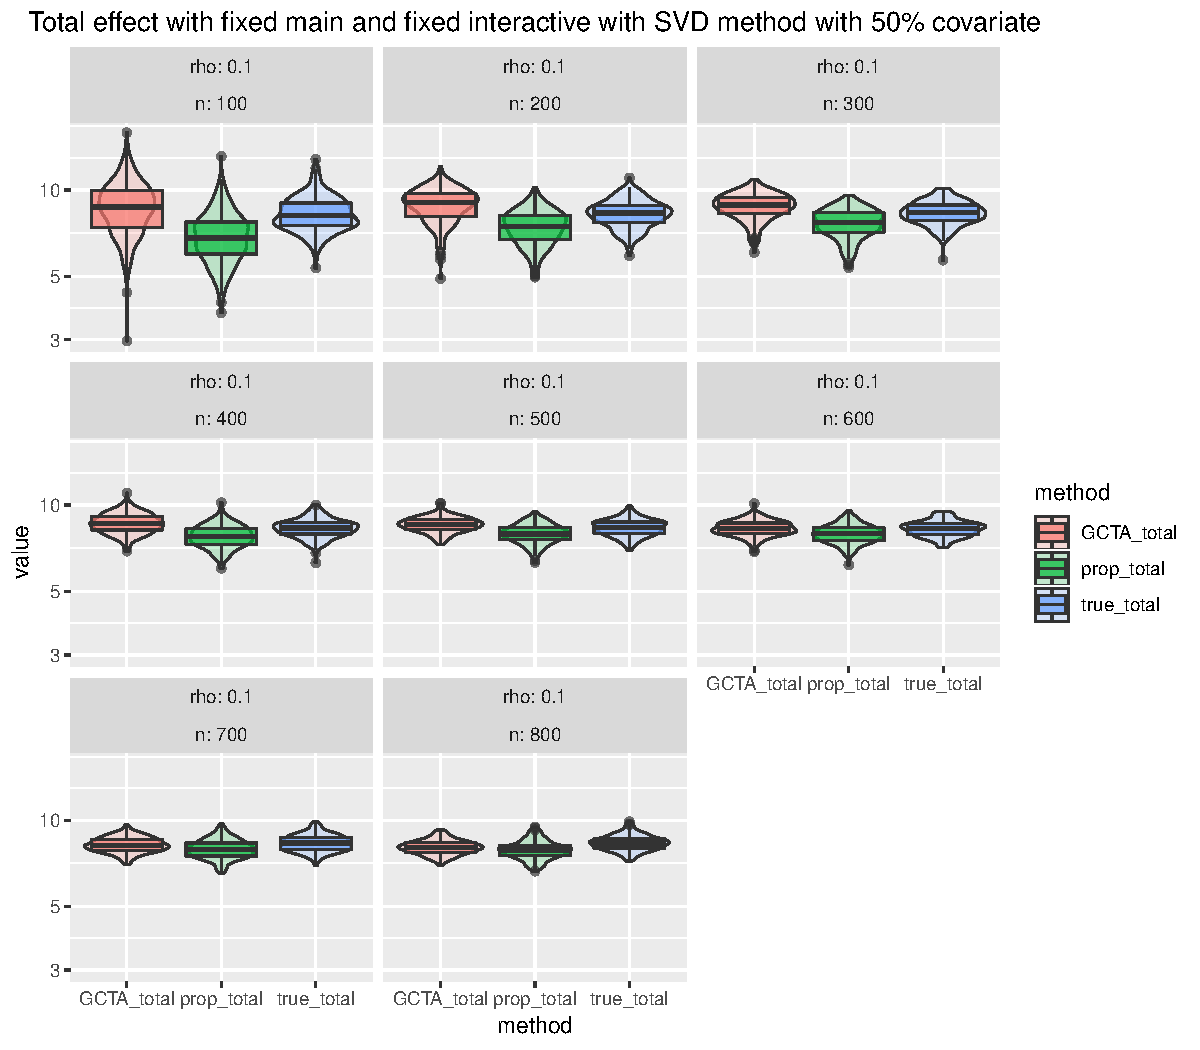
\includegraphics{./generate_graph_as_pdf/plot_chi_fixed_fixed_total_p_34_rho_0.1_0.9_n_100_800_svd_red_0.5.pdf}
\caption{Compound Stymmetry}
\end{figure}

\subsubsection{Autoregression AR(1)}\label{autoregression-ar1}

\[
  T = [T_1 \dots, T_p] ,~~~ T_i \sim \chi_{(1)}^2, ~~~ cov(T_i, T_j) = 2\rho^{2|i-j|},~~~ \forall  i \ne j, \rho = \{0.1, \dots, 0.9 \} 
\]

\begin{figure}
\centering
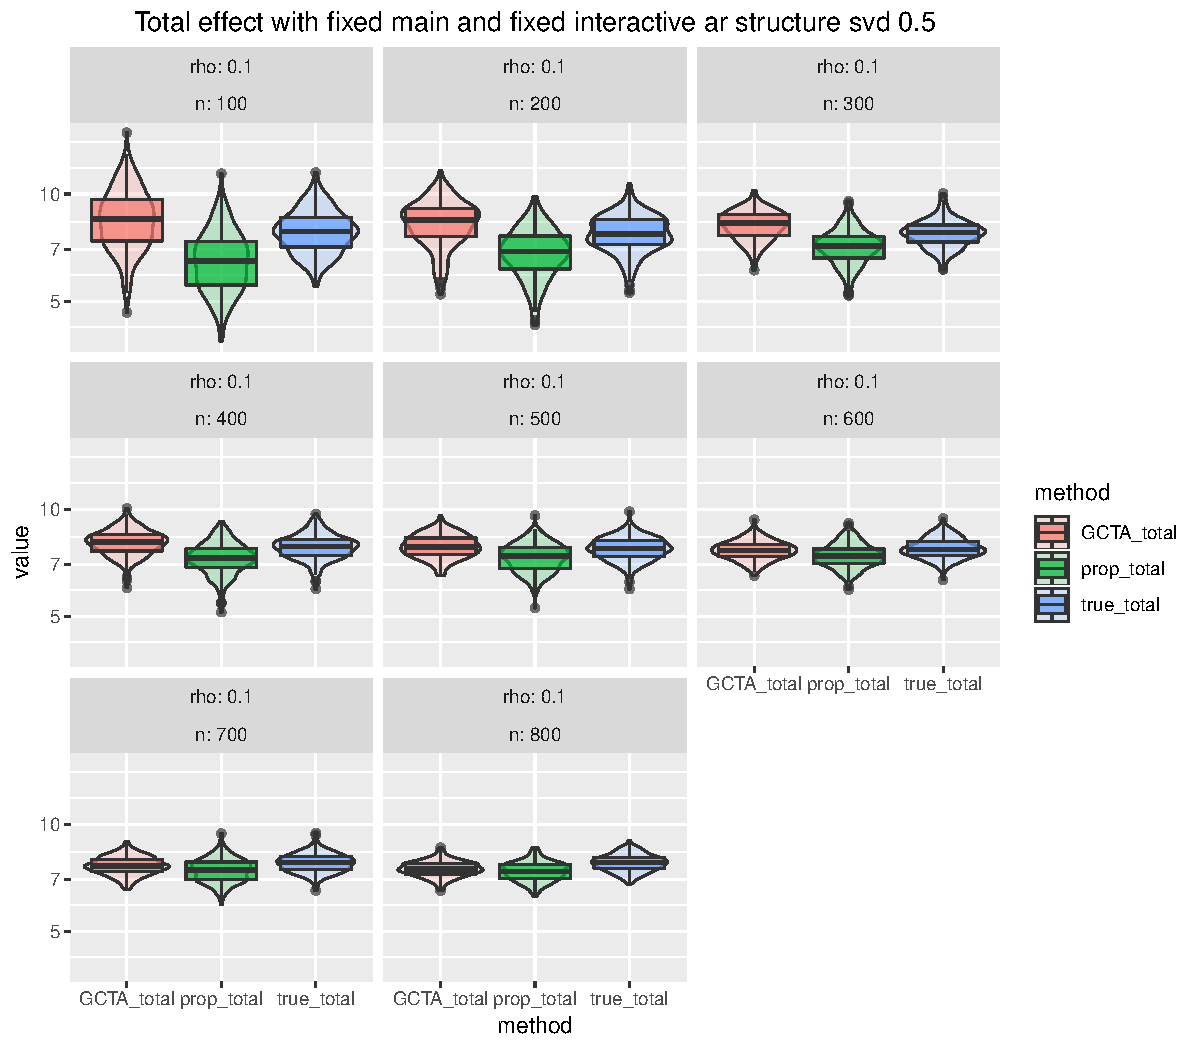
\includegraphics{./generate_graph_as_pdf/plot_chi_fixed_fixed_ar_chi_rho_0.1_0.9_n_100_800_p_34_svd_0.5.pdf}
\caption{AR(1)}
\end{figure}

\subsubsection{Unstructure}\label{unstructure}

\[
  T = [T_1 \dots, T_p] ,~~~ T_i \sim \chi_{(1)}^2, ~~~ cov(T_i, T_j) = \sigma_{ij}
\]

\begin{figure}
\centering
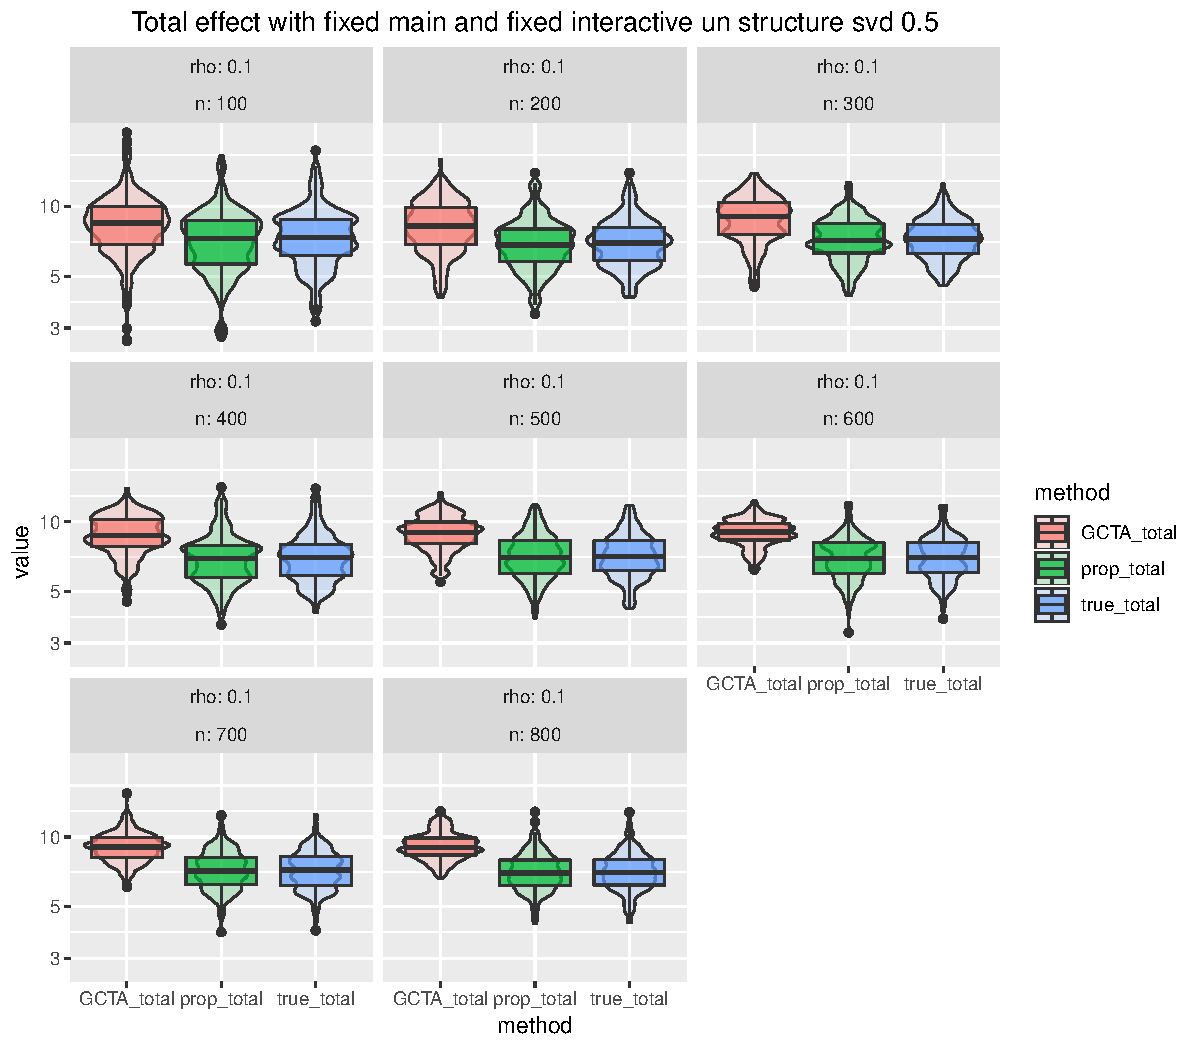
\includegraphics{./generate_graph_as_pdf/plot_chi_fixed_fixed_total_un_chi_rho_0.1_0.9_n_100_800_p_34_svd_0.5.pdf}
\caption{Unstructure}
\end{figure}

\newpage

\section{PCBs data simulation result}\label{pcbs-data-simulation-result}

We are using the PCBs data from the

\subsection{sample matrix of PCB data}\label{sample-matrix-of-pcb-data}

\subsubsection{A glimsp of the covariance
matrix}\label{a-glimsp-of-the-covariance-matrix}

\begin{table}[!h]

\caption{\label{tab:sub matrix of covariance of PCB}Covariance of PCB}
\centering
\resizebox{\linewidth}{!}{
\begin{tabular}[t]{l|r|r|r|r|r|r|r|r|r|r}
\hline
  & LBX028 & LBX066 & LBX074 & LBX105 & LBX118 & LBX156 & LBX157 & LBX167 & LBX044 & LBX049\\
\hline
LBX028 & 1.000 & 0.678 & 0.399 & 0.304 & 0.311 & 0.260 & 0.257 & 0.280 & 0.649 & 0.672\\
\hline
LBX066 & 0.678 & 1.000 & 0.665 & 0.721 & 0.694 & 0.502 & 0.509 & 0.629 & 0.327 & 0.333\\
\hline
LBX074 & 0.399 & 0.665 & 1.000 & 0.799 & 0.856 & 0.810 & 0.817 & 0.880 & 0.054 & 0.046\\
\hline
LBX105 & 0.304 & 0.721 & 0.799 & 1.000 & 0.974 & 0.689 & 0.707 & 0.840 & 0.046 & 0.040\\
\hline
LBX118 & 0.311 & 0.694 & 0.856 & 0.974 & 1.000 & 0.763 & 0.781 & 0.906 & 0.037 & 0.032\\
\hline
LBX156 & 0.260 & 0.502 & 0.810 & 0.689 & 0.763 & 1.000 & 0.989 & 0.890 & 0.004 & 0.000\\
\hline
LBX157 & 0.257 & 0.509 & 0.817 & 0.707 & 0.781 & 0.989 & 1.000 & 0.908 & -0.001 & -0.005\\
\hline
LBX167 & 0.280 & 0.629 & 0.880 & 0.840 & 0.906 & 0.890 & 0.908 & 1.000 & -0.015 & -0.019\\
\hline
LBX044 & 0.649 & 0.327 & 0.054 & 0.046 & 0.037 & 0.004 & -0.001 & -0.015 & 1.000 & 0.983\\
\hline
LBX049 & 0.672 & 0.333 & 0.046 & 0.040 & 0.032 & 0.000 & -0.005 & -0.019 & 0.983 & 1.000\\
\hline
\end{tabular}}
\end{table}

\subsubsection{Histgram of diagonal and off-diagonal elements of the
PCBs'sample
covariance}\label{histgram-of-diagonal-and-off-diagonal-elements-of-the-pcbssample-covariance}

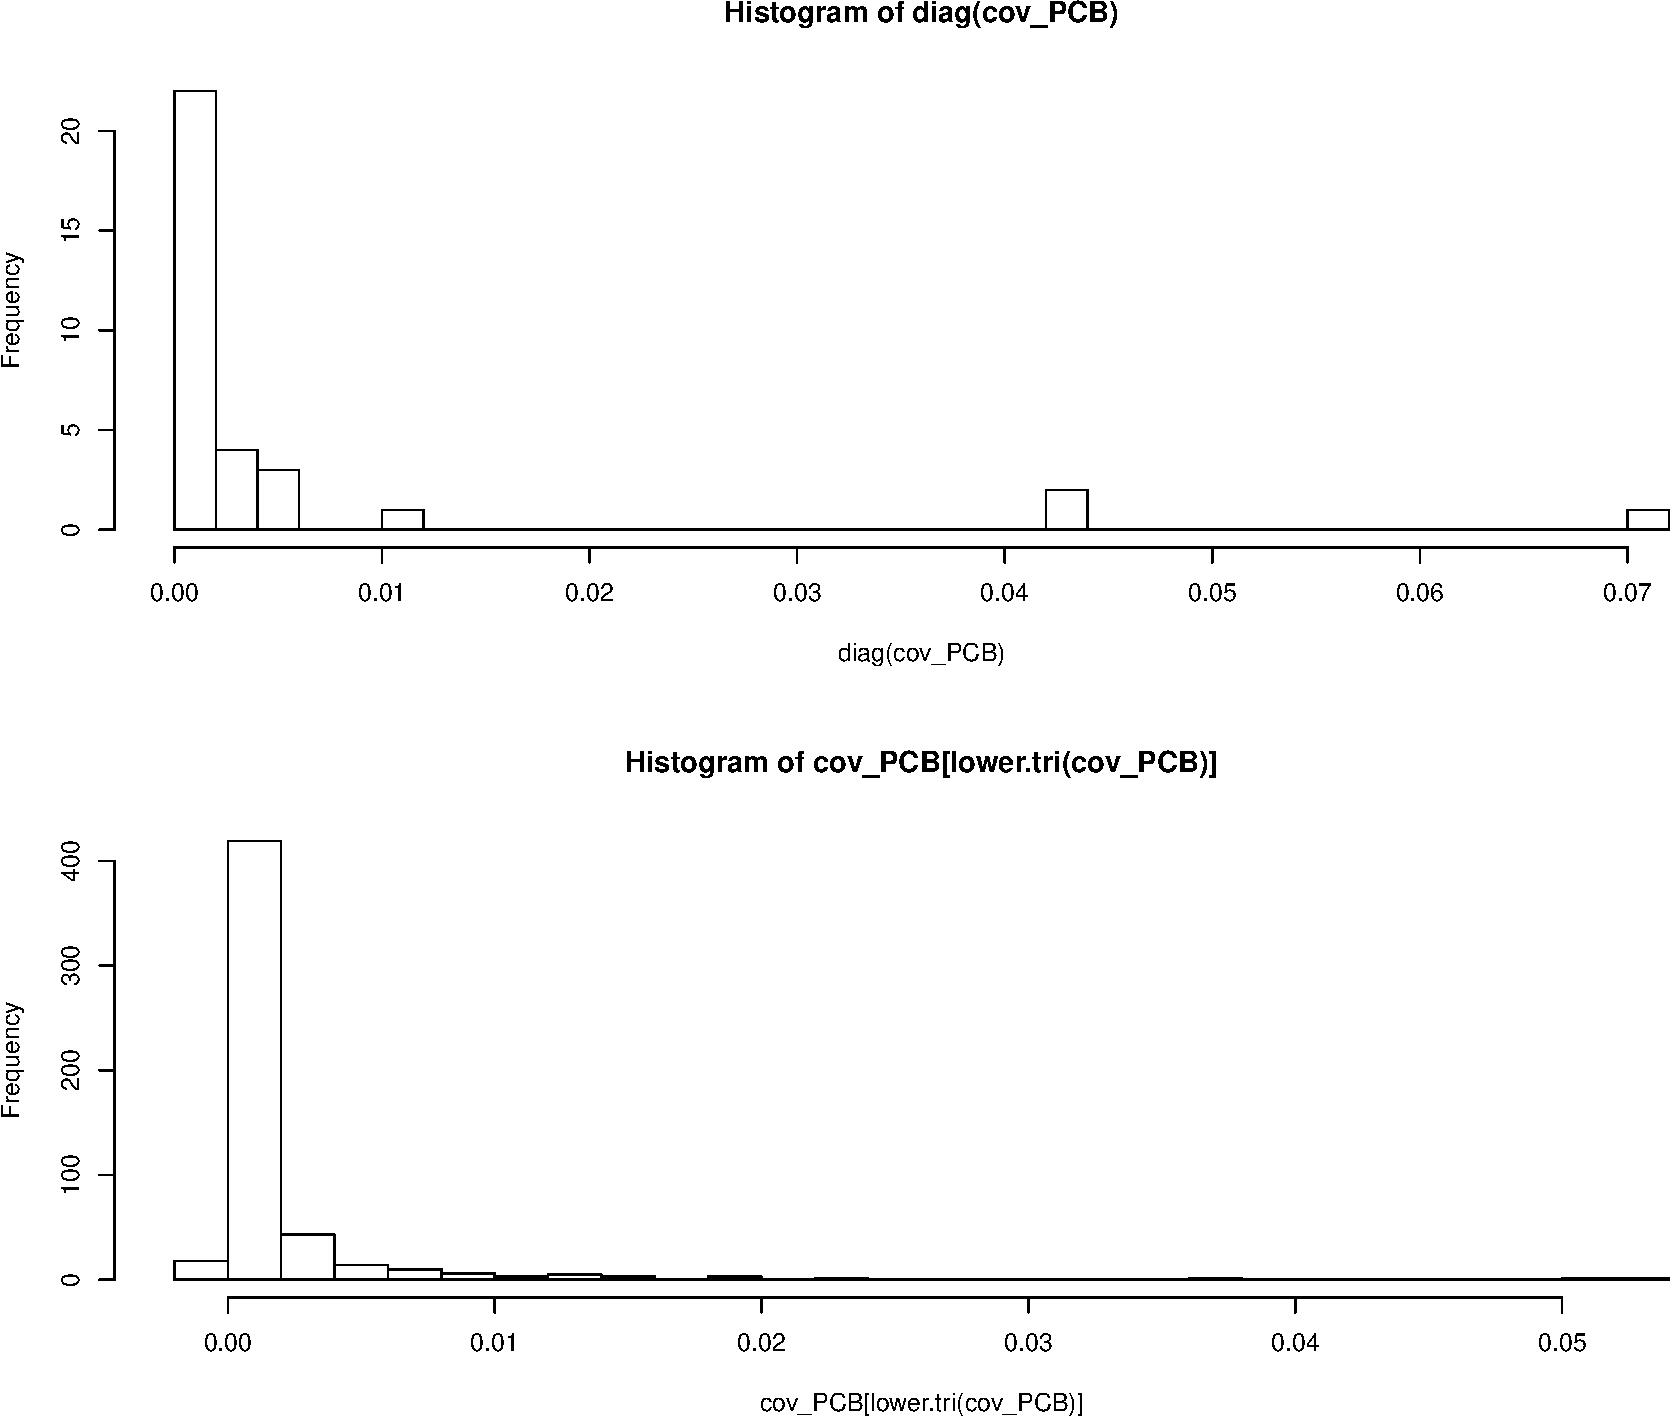
\includegraphics{SVD_dim_red_simulation_study_files/figure-latex/unnamed-chunk-1-1.pdf}

\subsubsection{Histgram of off-diagonal elements of the PCBs'sample
correlation-coefficient}\label{histgram-of-off-diagonal-elements-of-the-pcbssample-correlation-coefficient}

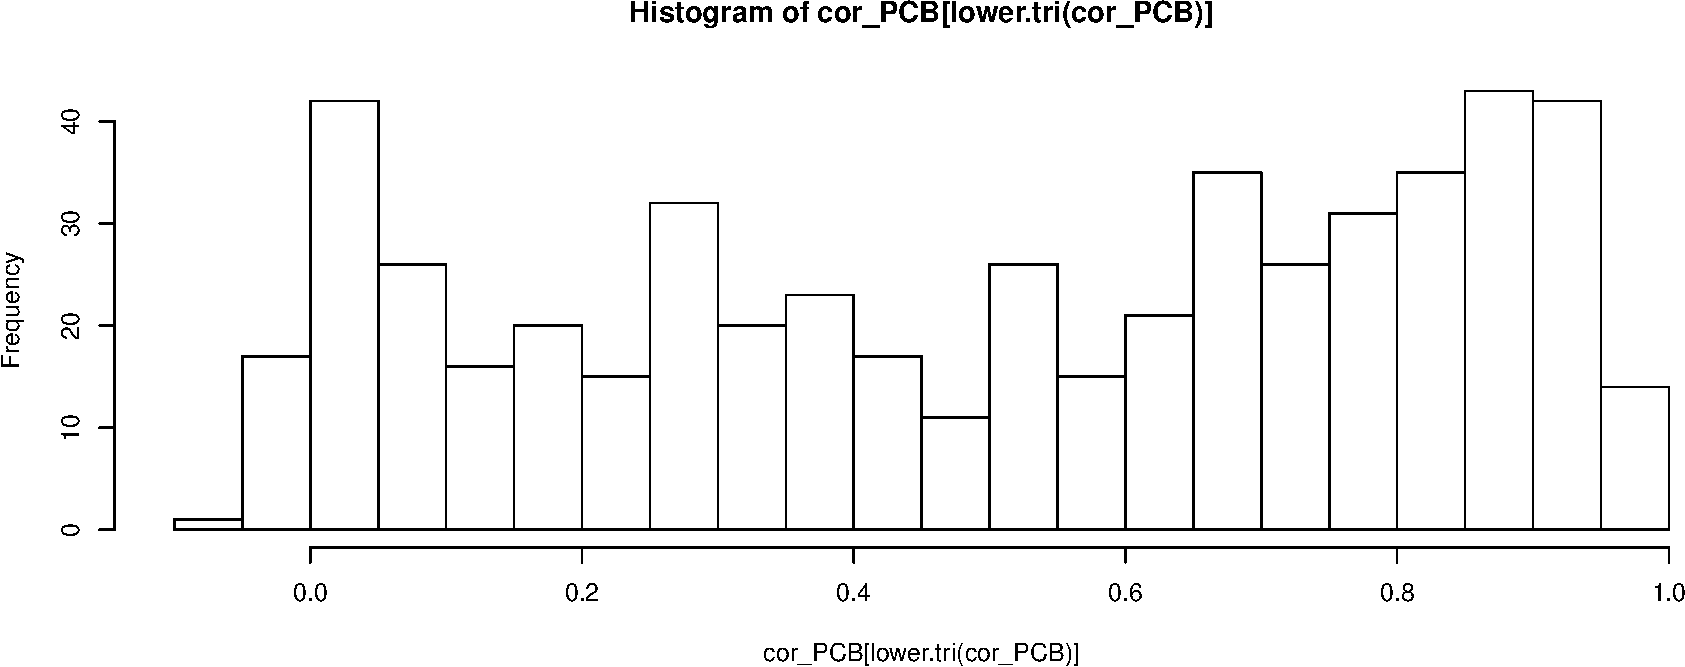
\includegraphics{SVD_dim_red_simulation_study_files/figure-latex/unnamed-chunk-2-1.pdf}

Based on the correlation coefficient values, it seems that there is no
an obvious pattern and the correlations are basically uniformly
distributed. Thus, the sample covariance of PCB is more likely to have
an unstructure structure.

\subsection{Simulation result}\label{simulation-result}

One thing about the PCB simulation is that we are using sub-sampling to
evaluate the performance of the PCB data.

\begin{figure}
\centering
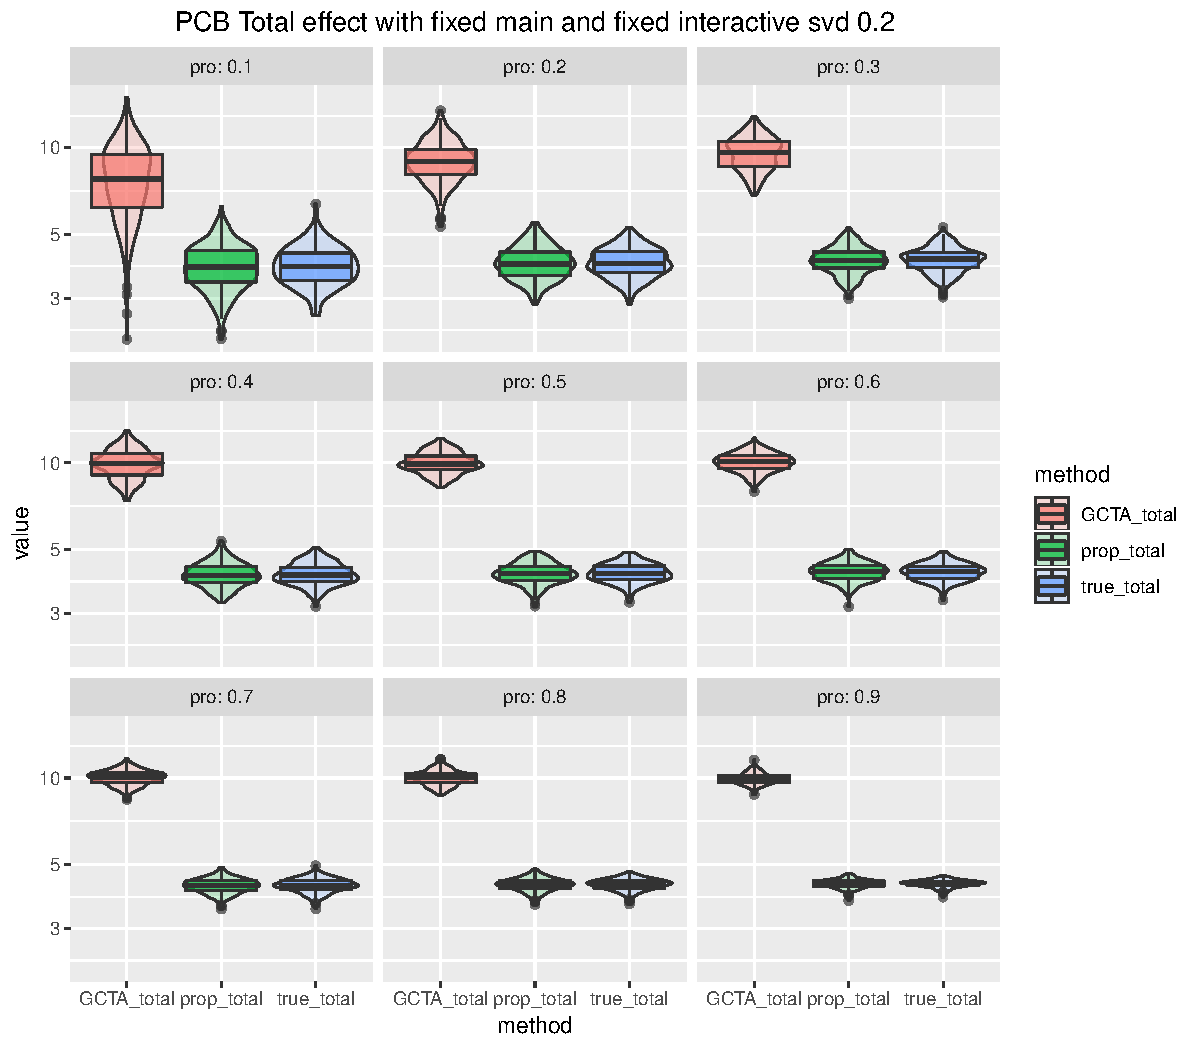
\includegraphics{./generate_graph_as_pdf/plot_PCB_fixed_fixed_pro_0.1_0.9_p_33_svd_0.2.pdf}
\caption{PCB with 0.2}
\end{figure}

\begin{figure}
\centering
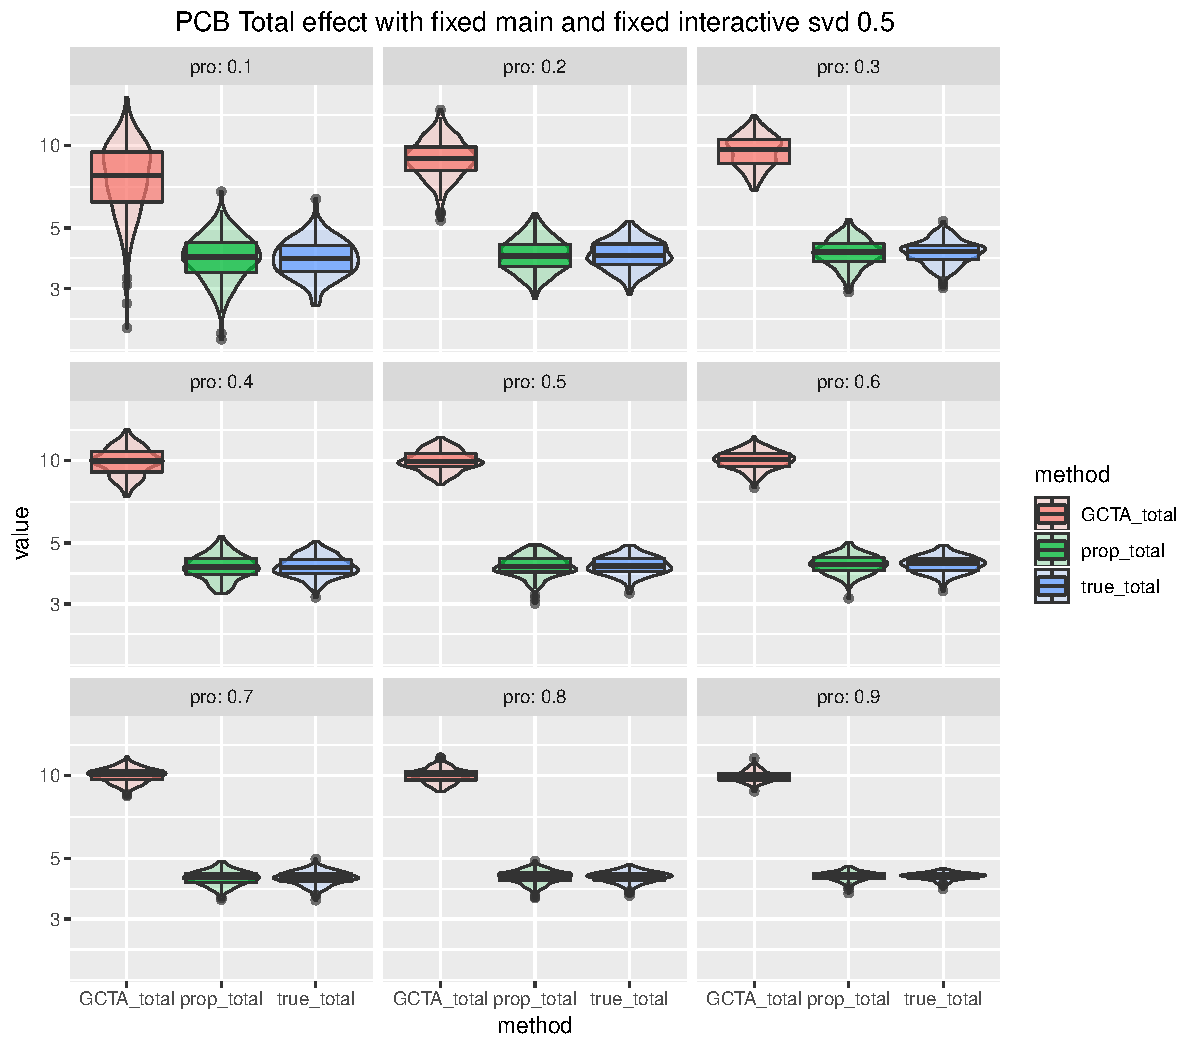
\includegraphics{./generate_graph_as_pdf/plot_PCB_fixed_fixed_pro_0.1_0.9_p_33_svd_0.5.pdf}
\caption{PCB with 0.5}
\end{figure}

\begin{figure}
\centering
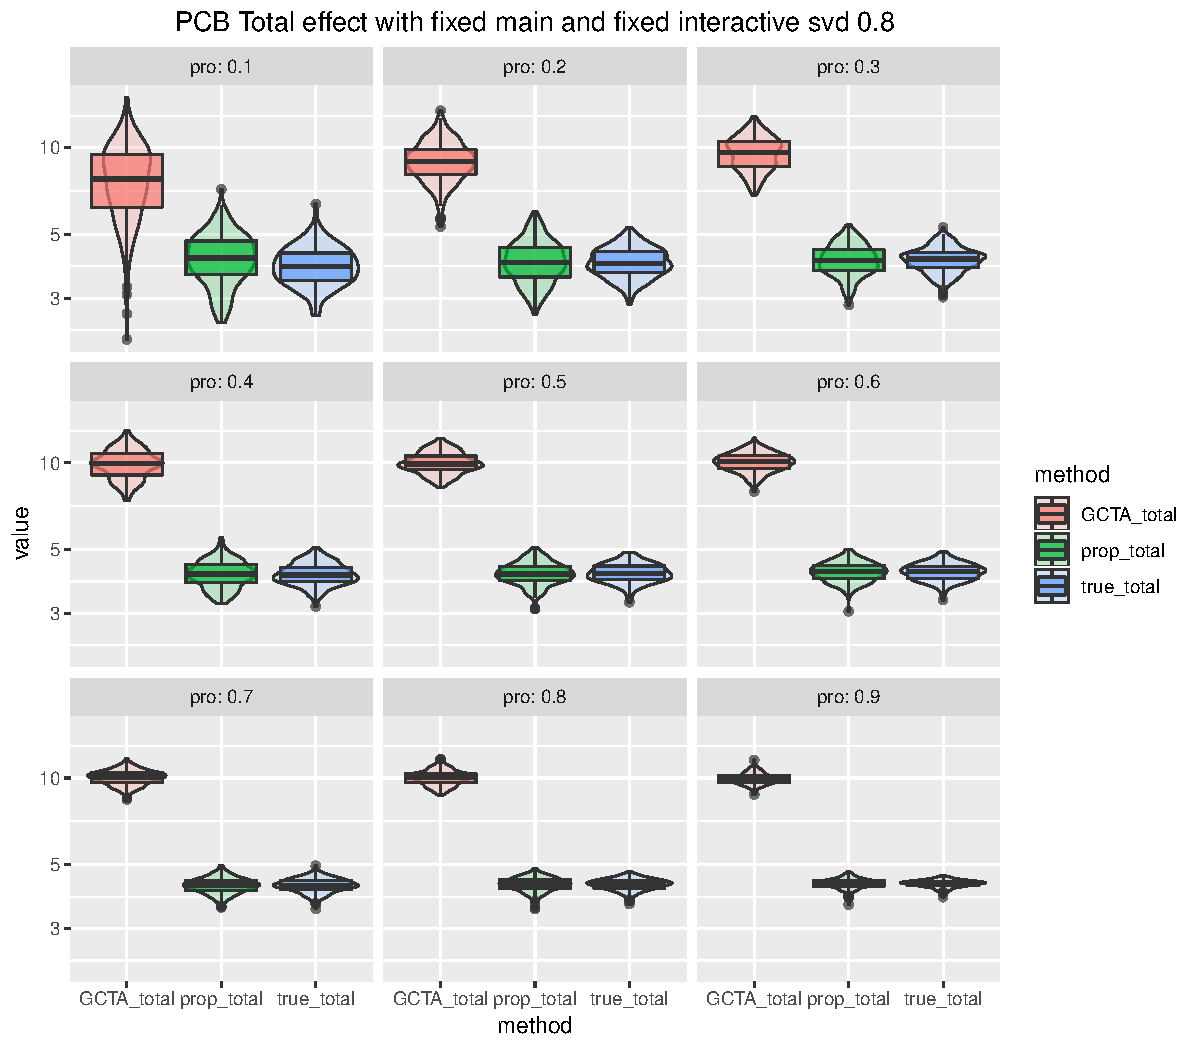
\includegraphics{./generate_graph_as_pdf/plot_PCB_fixed_fixed_pro_0.1_0.9_p_33_svd_0.8.pdf}
\caption{PCB with 0.8}
\end{figure}


\end{document}
